\documentclass{standalone}
\usepackage{tikz}

\begin{document}



\tikzset{every picture/.style={line width=0.75pt}} %set default line width to 0.75pt        

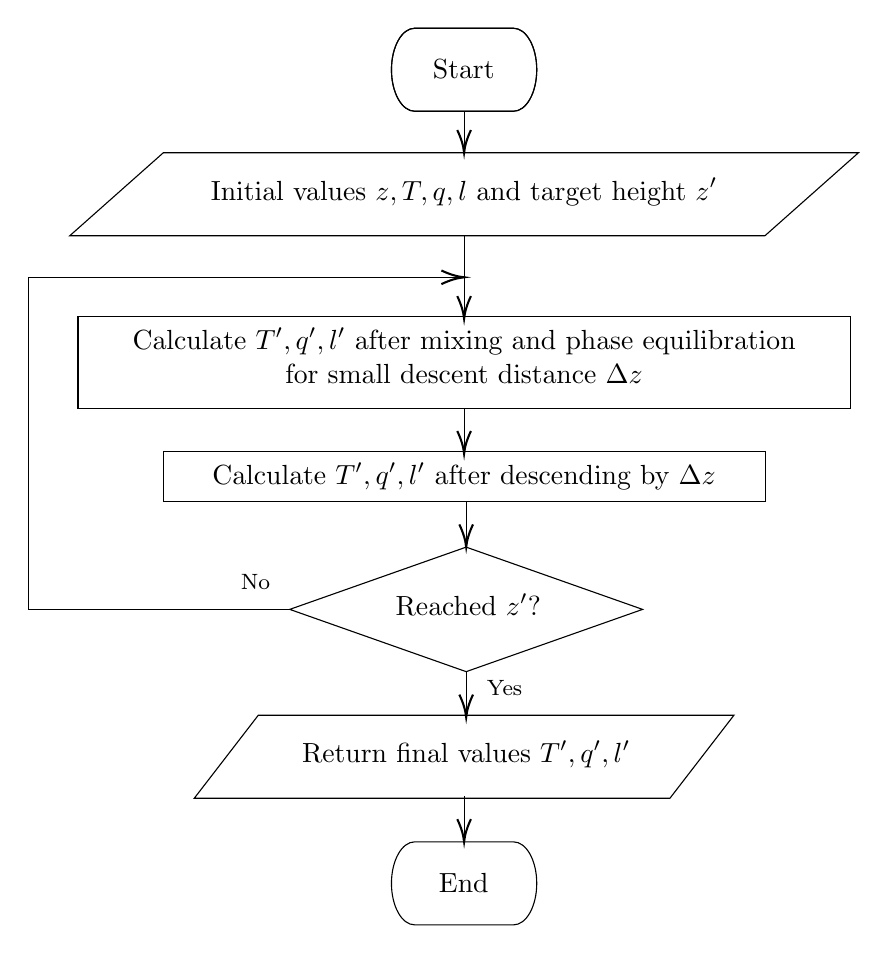
\begin{tikzpicture}[x=0.75pt,y=0.75pt,yscale=-1,xscale=1]
%uncomment if require: \path (0,504); %set diagram left start at 0, and has height of 504

%Flowchart: Terminator [id:dp08567911049849242] 
\draw   (296.2,30) -- (343.8,30) .. controls (349.99,30) and (355,38.95) .. (355,50) .. controls (355,61.05) and (349.99,70) .. (343.8,70) -- (296.2,70) .. controls (290.01,70) and (285,61.05) .. (285,50) .. controls (285,38.95) and (290.01,30) .. (296.2,30) -- cycle ;
%Shape: Parallelogram [id:dp7440666445542639] 
\draw   (175.08,90) -- (510,90) -- (464.92,130) -- (130,130) -- cycle ;
%Straight Lines [id:da8613041389593643] 
\draw    (320,70) -- (320,88) ;
\draw [shift={(320,90)}, rotate = 270] [color={rgb, 255:red, 0; green, 0; blue, 0 }  ][line width=0.75]    (10.93,-3.29) .. controls (6.95,-1.4) and (3.31,-0.3) .. (0,0) .. controls (3.31,0.3) and (6.95,1.4) .. (10.93,3.29)   ;
%Straight Lines [id:da5516964412362506] 
\draw    (320,130) -- (320,168) ;
\draw [shift={(320,170)}, rotate = 270] [color={rgb, 255:red, 0; green, 0; blue, 0 }  ][line width=0.75]    (10.93,-3.29) .. controls (6.95,-1.4) and (3.31,-0.3) .. (0,0) .. controls (3.31,0.3) and (6.95,1.4) .. (10.93,3.29)   ;
%Straight Lines [id:da07493245791577552] 
\draw    (320,213) -- (320,233) ;
\draw [shift={(320,235)}, rotate = 270] [color={rgb, 255:red, 0; green, 0; blue, 0 }  ][line width=0.75]    (10.93,-3.29) .. controls (6.95,-1.4) and (3.31,-0.3) .. (0,0) .. controls (3.31,0.3) and (6.95,1.4) .. (10.93,3.29)   ;
%Flowchart: Decision [id:dp12562758914817684] 
\draw   (321,280) -- (406,310) -- (321,340) -- (236,310) -- cycle ;
%Straight Lines [id:da7410521308863762] 
\draw    (321,258) -- (321,278) ;
\draw [shift={(321,280)}, rotate = 270] [color={rgb, 255:red, 0; green, 0; blue, 0 }  ][line width=0.75]    (10.93,-3.29) .. controls (6.95,-1.4) and (3.31,-0.3) .. (0,0) .. controls (3.31,0.3) and (6.95,1.4) .. (10.93,3.29)   ;
%Straight Lines [id:da42305541202637564] 
\draw    (318,150) -- (110,150) -- (110,310) -- (236,310) ;
\draw [shift={(320,150)}, rotate = 180] [color={rgb, 255:red, 0; green, 0; blue, 0 }  ][line width=0.75]    (10.93,-3.29) .. controls (6.95,-1.4) and (3.31,-0.3) .. (0,0) .. controls (3.31,0.3) and (6.95,1.4) .. (10.93,3.29)   ;
%Straight Lines [id:da5975737713245242] 
\draw    (321,340) -- (321,360) ;
\draw [shift={(321,362)}, rotate = 270] [color={rgb, 255:red, 0; green, 0; blue, 0 }  ][line width=0.75]    (10.93,-3.29) .. controls (6.95,-1.4) and (3.31,-0.3) .. (0,0) .. controls (3.31,0.3) and (6.95,1.4) .. (10.93,3.29)   ;
%Flowchart: Terminator [id:dp8795625942273118] 
\draw   (296.2,30) -- (343.8,30) .. controls (349.99,30) and (355,38.95) .. (355,50) .. controls (355,61.05) and (349.99,70) .. (343.8,70) -- (296.2,70) .. controls (290.01,70) and (285,61.05) .. (285,50) .. controls (285,38.95) and (290.01,30) .. (296.2,30) -- cycle ;
%Flowchart: Terminator [id:dp591794969904871] 
\draw   (296.2,422) -- (343.8,422) .. controls (349.99,422) and (355,430.95) .. (355,442) .. controls (355,453.05) and (349.99,462) .. (343.8,462) -- (296.2,462) .. controls (290.01,462) and (285,453.05) .. (285,442) .. controls (285,430.95) and (290.01,422) .. (296.2,422) -- cycle ;
%Shape: Parallelogram [id:dp18570385722047877] 
\draw   (220.84,361) -- (450,361) -- (419.16,401) -- (190,401) -- cycle ;
%Straight Lines [id:da1670574143718757] 
\draw    (320,400) -- (320,420) ;
\draw [shift={(320,422)}, rotate = 270] [color={rgb, 255:red, 0; green, 0; blue, 0 }  ][line width=0.75]    (10.93,-3.29) .. controls (6.95,-1.4) and (3.31,-0.3) .. (0,0) .. controls (3.31,0.3) and (6.95,1.4) .. (10.93,3.29)   ;

% Text Node
\draw (319.84,44) node [anchor=north] [inner sep=0.75pt]   [align=left] {Start};
% Text Node
\draw (320,101) node [anchor=north] [inner sep=0.75pt]   [align=left] {Initial values $\displaystyle z,T,q,l$ and target height $\displaystyle z'$};
% Text Node
\draw    (134,169) -- (506,169) -- (506,213) -- (134,213) -- cycle  ;
\draw (320,173) node [anchor=north] [inner sep=0.75pt]   [align=left] {\begin{minipage}[lt]{250.38pt}\setlength\topsep{0pt}
\begin{center}
 Calculate $\displaystyle T',q',l'$ after mixing and phase equilibration\\for small descent distance $\displaystyle \Delta z$
\end{center}

\end{minipage}};
% Text Node
\draw    (175,234) -- (465,234) -- (465,258) -- (175,258) -- cycle  ;
\draw (320,238) node [anchor=north] [inner sep=0.75pt]   [align=left] {\begin{minipage}[lt]{194.29pt}\setlength\topsep{0pt}
\begin{center}
Calculate $\displaystyle T',q',l'$ after descending by $\displaystyle \Delta z$ 
\end{center}

\end{minipage}};
% Text Node
\draw (322,301) node [anchor=north] [inner sep=0.75pt]   [align=left] {\begin{minipage}[lt]{60.39pt}\setlength\topsep{0pt}
\begin{center}
Reached $\displaystyle z'$?
\end{center}

\end{minipage}};
% Text Node
\draw (219.5,292) node [anchor=north] [inner sep=0.75pt]   [align=left] {\begin{minipage}[lt]{13.15pt}\setlength\topsep{0pt}
\begin{center}
{\footnotesize No}
\end{center}

\end{minipage}};
% Text Node
\draw (339.5,343) node [anchor=north] [inner sep=0.75pt]   [align=left] {\begin{minipage}[lt]{16.03pt}\setlength\topsep{0pt}
\begin{center}
{\footnotesize Yes}
\end{center}

\end{minipage}};
% Text Node
\draw (319.84,436) node [anchor=north] [inner sep=0.75pt]   [align=left] {End};
% Text Node
\draw (321,372) node [anchor=north] [inner sep=0.75pt]   [align=left] {Return final values $\displaystyle T',q',l'$};


\end{tikzpicture}

\end{document}